\section{Status of J-PARC T59 experiment}
We had submitted a proposal of a test experiment to J-PARC in April 2014 to test a new detector with a water target, WAGASCI, at the neutrino monitor hall, and the proposal was approved as J-PARC T59.
The project contains the side and downstream muon range detectors as well.

The first WAGASCI module has been constructed in 2016 and installed at the on-axis position in front of the T2K INGRID detector for the commissioning and the first cross section measurement as a part of the T2K experiment.
The INGRID electronics boards are used to read the signal.
The light yield measured with muons produced by the interaction of neutrinos
in the hall wall, shown in Fig.~\ref{fig:wmlight}, is sufficiently high to get good hit efficiency.  
%
\begin{figure}[tbh]
\begin{center}
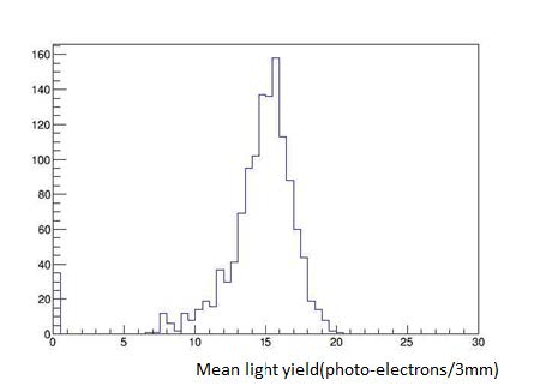
\includegraphics[width=0.5\linewidth]{fig/wmlight.pdf}
\end{center}
\caption{Light yield for muons produced by the interaction of neutrinos
  in the hall wall. Average light yields for each channel are plotted.
}
\label{fig:wmlight}
\end{figure}
A track search algorithm based on the cellular automaton has been developed using the software tools by the T2K INGRID. 
Examples of observed events are shown in Fig.~\ref{fig:onaxis_eventdisplay}
The tracking efficiency in 2-dimensional projected plane was evaluated by comparing the reconstructed track
in the WAGASCI module and the INGRID module and shown in Fig.\ref{fig:wmefficiency}.
Note that that the tracking efficiency for high angle ($>70\deg$) is not evaluated because of the acceptance
of the INGRID module, not because of the limitation of the WAGASCI module.
\begin{figure}[tbhp]
\begin{center}
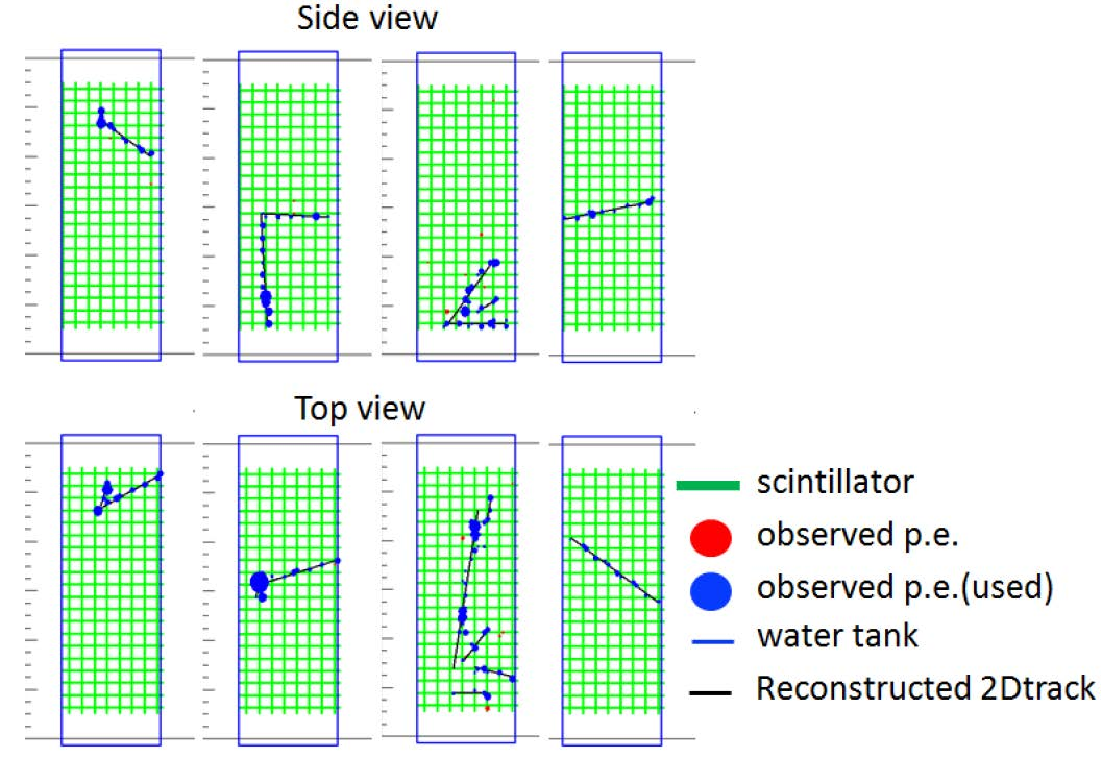
\includegraphics[width=\textwidth]{fig/wagascieventdisp.pdf}
%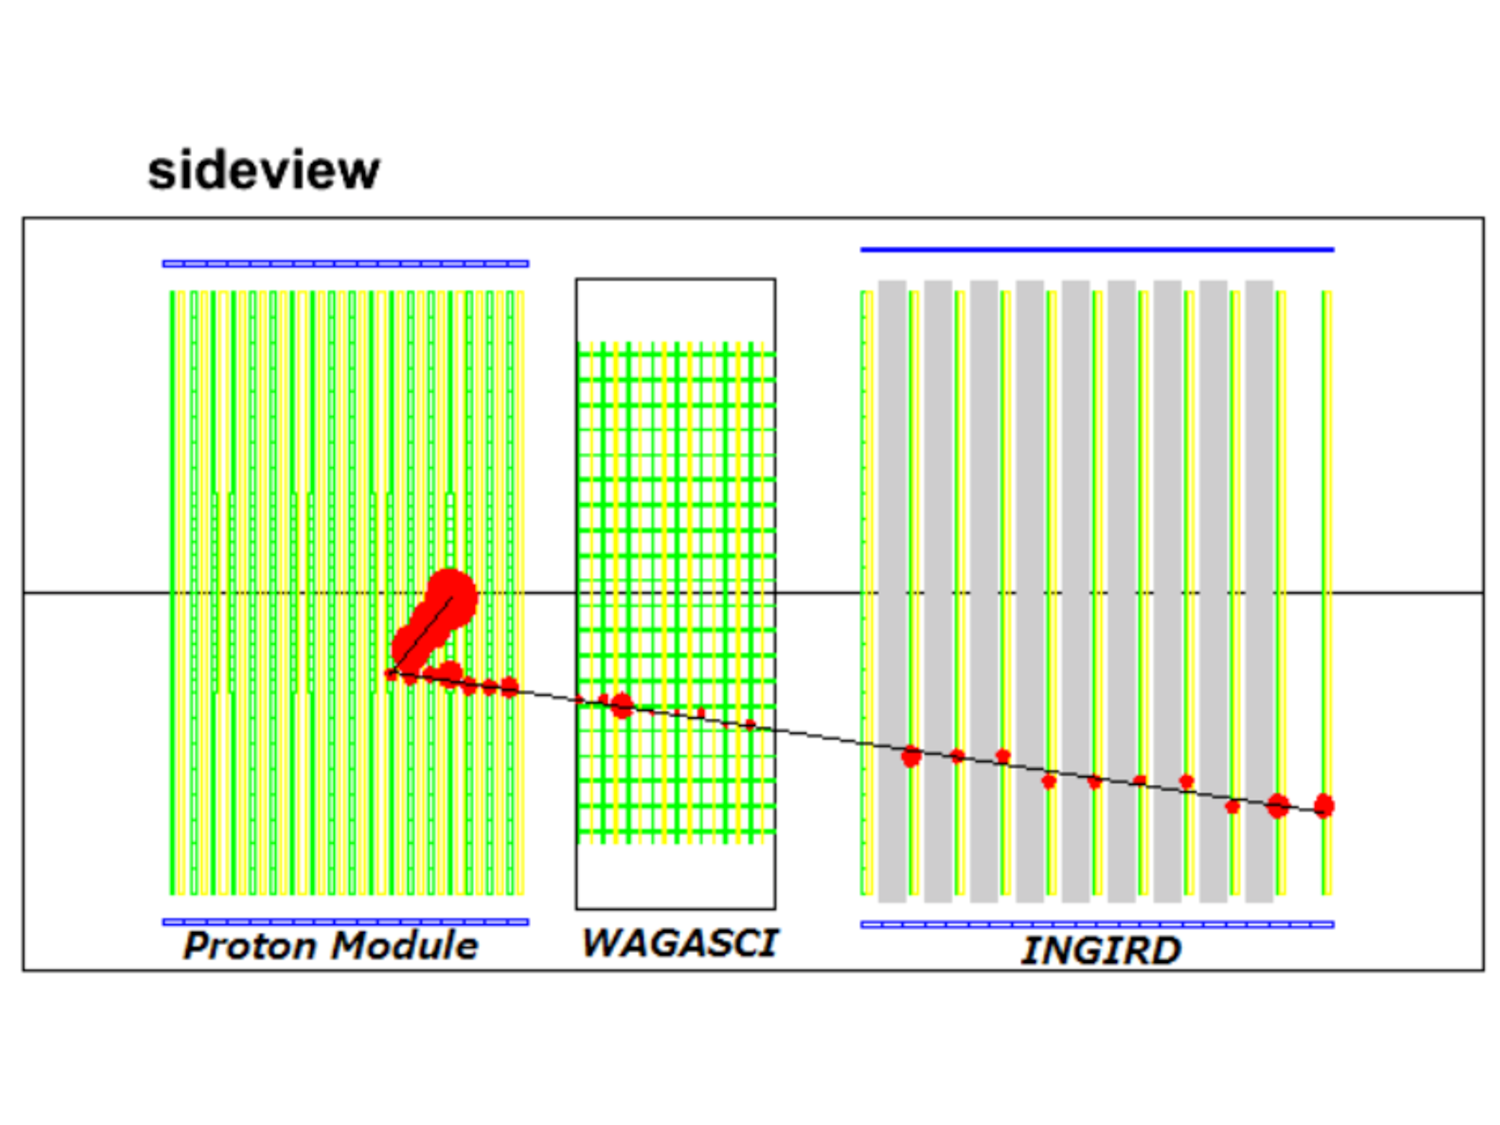
\includegraphics[width=0.8\linewidth]{fig/t59_event_display_oct_dec_2017.pdf}
% \includegraphics[width=0.8\linewidth]{fig/all_detector2.pdf}
\end{center}
\caption{
  Example event displays of the WAGASCI module at on-axis.
  The reconstructed tracks are overlaid.}
\label{fig:onaxis_eventdisplay}
%  t59_event_display_oct_dec_2017}
\end{figure}
%
\begin{figure}[tbhp]
  \begin{center}
   \begin{subfigure}{0.48\textwidth}
     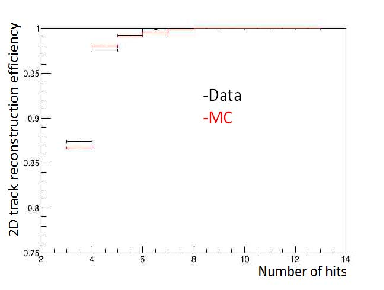
\includegraphics[width=\linewidth]{fig/wmeffvshit.pdf}
    \end{subfigure}
  \begin{subfigure}{0.48\textwidth}
      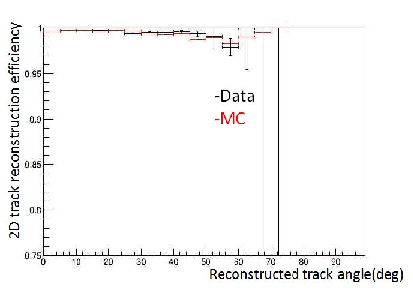
\includegraphics[width=\linewidth]{fig/wmeffvsangle.pdf}
    \end{subfigure}    
    \end{center}
  \caption{2D track reconstruction efficiency as a function of number of hits (left) and track angle (right).
  Here the track angle is the one reconstructed by the INGRID module.}
\label{fig:wmefficiency}
\end{figure}

In 2017 Autumn, the construction of the second WAGASCI module and the dedicated electronics board were completed.
The module and the electronics were install to the B2 floor together with the T2K proton module and the INGRID
module as shown in Fig.~\ref{fig:det_confg_oct_dec2017}.
The proton module is to be used as the entering muon veto and also for the comparison of interaction between CH and Water.
The INGRID module is for the temporary muon detector with limited acceptance for this period.
The detector was commissioned and is in operation to take data with the antineutrino beam during the T2K beam time from October.

 \begin{figure}[tbhp]
 \begin{center}
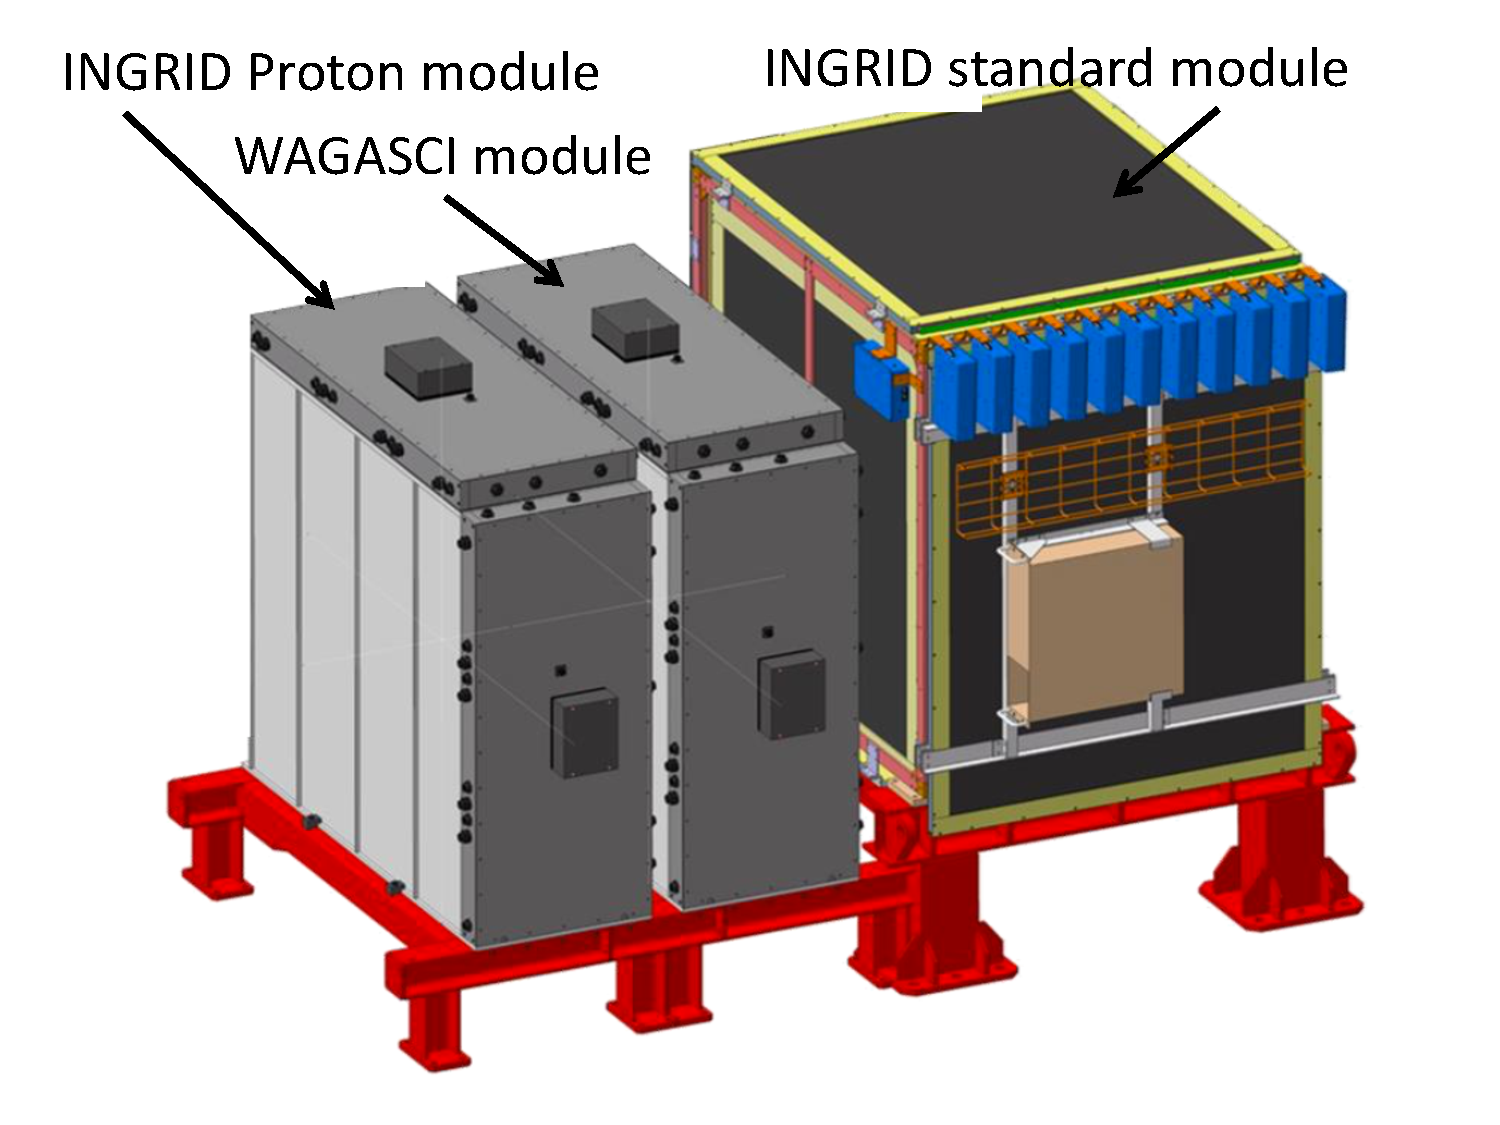
\includegraphics[width=0.5\linewidth]{fig/t59_det_config_oct_dec_2017.pdf}
 \end{center}
 \caption{
 J-PARC T59 detector configuration in October 2017.
 }
 \label{fig:det_confg_oct_dec2017}
 \end{figure}

The production of the components of the side muon range detectors has been completed and now the detectors
are being assembled at the Yokohama National University.
These detectors will be installed sometime from January to June, 2018 when T2K is not running.

The Baby MIND detector was transported from CERN to Japan in December, 2017.
It will be installed and commissioned in Jan.-Feb. 2018 and T59 will take the neutrino-induced muon data in April and May.

%Fist, the start time of neutrino beam measurement is changed from December 2015 to October 2017, and the requested neutrino beam is changed from $1\times10^{21}$ POT of $\nu$ beam to $0.8\times10^{21} $POT of anti-$\nu$ beam. 
% Second, the detector configuration is changed. In the original proposal, central neutrino detector are expected to be surrounded by newly developed muon-range detectors (MRDs), but we will use spare neutrino detectors of the T2K experiment instead of them during neutrino beam measurement from October to December 2017. Construction of the newly developed MRDs, Baby-MIND and Side-MRD, is in progress, and they will be installed to the both sides and the downstream of the central neutrino detector from January to March 2018. Then, we will resume neutrino beam measurements from March 2018 and will take the neutrino beam data until May 2018.


%\subsection{On-axis beam measurement with Prototype detector}
%Add INGRID water module measurement here.

%\subsection{Plans from October 2017 to May 2018}
%J-PARC MR will extract its proton beam to T2K neutrino beam-line from October to December 2017, and, from March to May 2018. 
%T2K experiment will produce anti-neutrino beam and will accumulate $\sim8\times10^{20}$ POT data during the above period.


% J-PARC T59 will perform neutrino beam measurements on the B2 floor of the T2K near neutrino detector hall during the above period to test basic performances of the WAGASCI detector and new electronics. During the beam measurements from October to December 2017, one WAGASCI module will be placed between spare neutrino detectors of the T2K experiment, INGRID Proton module and INGRID standard module. 
 % as shown in Fig. \ref{fig:det_config_oct_dec2017}.
% Detector location on the B2 floor of T2K near detector hall is shown in Fig. \ref{fig:det_loc_oct_dec2017}. 
%Here, the INGRID Proton module is used as a charged particle VETO detector and, the INGRID standard module is used as a downstream muon detector. 
%We had submitted a proposal to use these spare neutrino detectors for the T59 neutrino beam measurements to the T2K collaboration, and we got an approval from T2K. 


 
% \begin{figure}[tbh]
% \begin{center}
% 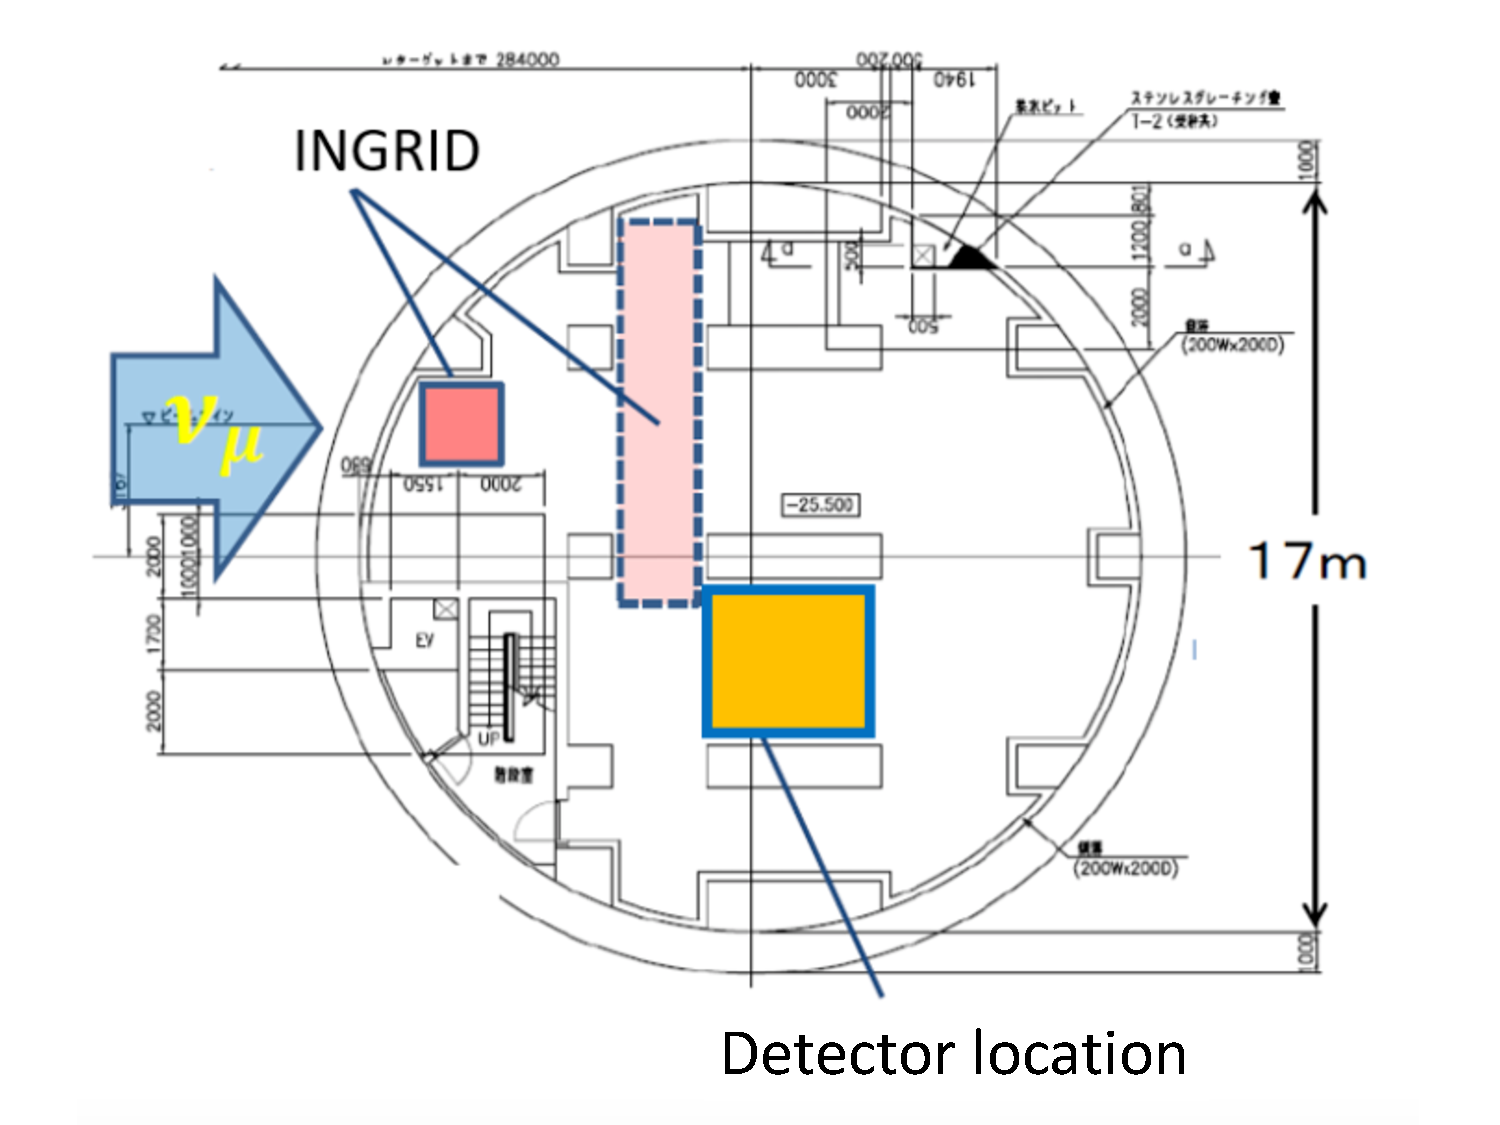
\includegraphics[width=0.8\linewidth]{fig/t59_det_location_oct_dec_2017.pdf}
% \end{center}
% \caption{
% J-PARC T59 detector location from Oct. to Dec. 2017
% }
% \label{fig:det_loc_oct_dec2017}
% \end{figure}


%During the beam measurements from March to May 2018, Baby-MIND and two side muon-range detector (Side-MRD) modules will be installed on the downstream and the both sides of the WAGASCI detector, as shown in Fig. \ref{fig:det_config_mar_may2018}, to increase angular acceptance for secondary charged particles from neutrino interactions.
 
%\begin{figure}[tbh]
%\begin{center}
%
\includegraphics[width=0.8\linewidth]{fig/tmp.pdf}
% \includegraphics[width=0.8\linewidth]{fig/all_detector2.pdf}
%\end{center}
%\caption{
%J-PARC T59 detector configuration with Baby-MIND and two Side-MRD modules from Mar. to May 2018.
%(Need to prepare the figure.)}
%\label{fig:det_config_mar_may2018}
%\end{figure}


%Expected number of neutrino events in the WAGASCI detector during the above beam period is evaluated with Monte Carlo simulations. 
%Neutrino beam flux at the detector location is simulated by T2K neutrino flux generator, JNUBEAM, neutrino interactions with target materials are simulated by a neutrino interaction simulator, NEUT, detector responses are simulated using GEANT4-based simulation. 
%The neutrino flux at the detector location, 1.5 degrees away from the J-PARC neutrino beam axis, is shown in Figure \ref{fig:b2flux}, and its mean neutrino energy is around 0.68 GeV.


%To perform the detector performance test, the following event selections are applied to the data. 
%First, track reconstructions are performed in the WAGASCI detector, and the reconstructed vertex is required to be inside a defined fiducial volume, $80 \times80 \times 32$ cm$^{3}$ region at the center of the detector, to reduce contamination from external backgrounds. 
%Second, at least one charged particle is required to reach to INGRID standard module or Side-MRD modules, and it makes more than two hits in these sub-detectors. 
%With the event selection, expected numbers of the neutrino-candidate events during the beam period are summarized in Table 1. 
%Using the data, we will test the detector performance with $\sim3$\% statistical uncertainties.








